\chapter{Contexte Général}

\section*{Introduction}
\addcontentsline{toc}{section}{Introduction}
Ce chapitre offre un aperçu général de SEGULA Technologies, en mettant en évidence son historique, son chiffre d'affaires, ses secteurs d'activité ainsi que sa clientèle, notamment le groupe Stellantis. Il explore également le cycle de vie du véhicule au sein de l'usine, ses différents types, le processus de fabrication et les outils de conception utilisés.

\section{Présentation de l'organisme d'accueil}

\subsection{Groupe SEGULA}
Le groupe SEGULA Technologies est présent dans plus de 30 pays, avec 140 implantations à travers le monde. Il privilégie une relation de proximité avec ses clients, grâce aux compétences de ses 12 000 à 15 000 collaborateurs. Ingénieriste de premier plan, plaçant l'innovation au cœur de sa stratégie, SEGULA Technologies mène des projets d'envergure, couvrant l'ensemble des phases, des études jusqu'à l'industrialisation et la production.


\begin{figure}[H]
    \centering
    
\includegraphics[width=0.75\linewidth]{chapters/SEGULA_Technologies_logo.png}
    \caption{Logo de SEGULA Technologies}
    \label{fig:placeholder}
\end{figure}

Fondé en 1985, SEGULA Technologies est un groupe d'ingénierie et de conseil en innovation dirigé par un directoire présidé par Franck Ghrenassia. Son siège social est situé à Nanterre. Initialement centré sur l'industrie automobile, qui reste son principal secteur d'activité, le groupe s'est diversifié dans d'autres domaines tels que l'aéronautique, l'énergie, le ferroviaire ou le naval, notamment par des acquisitions stratégiques.

SEGULA Technologies accompagne ses clients tout au long des projets techniques, depuis les phases d'études, de management et de conception, jusqu'à la fiabilisation, l'industrialisation et la production, en fournissant des solutions sous forme de conseils ou de collaborateurs spécialisés.

\begin{figure}
    \centering
    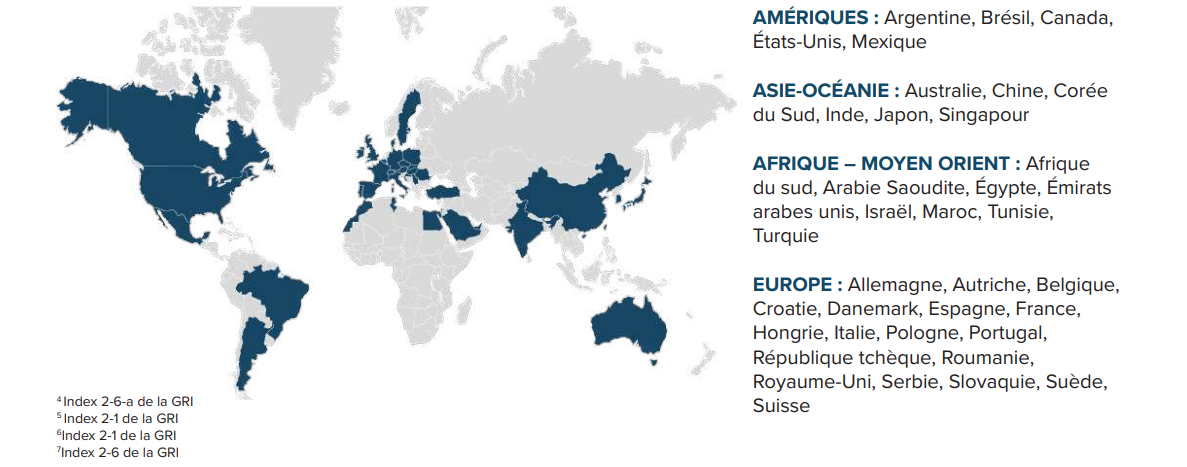
\includegraphics[width=1\linewidth]{Implantation.png}
    \caption{Implantation de SEGULA Technologies à l’échelle internationale}
\end{figure}
\subsection{Fiche signalétique de l'entreprise}
Le tableau ci-dessous présente les données clés du groupe SEGULA Technologies.

\begin{table}[H]
    \centering
    \begin{tabular}{|p{4cm}|p{10cm}|}
        \hline
        \textbf{Raison sociale} & SEGULA Technologies \\ \hline
        \textbf{Forme juridique} & Société par Actions Simplifiée (SAS) \\ \hline
        \textbf{Activité} & Groupe d'ingénierie et de conseil en innovation \\ \hline
        \textbf{Date de création} & 1985, France \\ \hline
        \textbf{Implantations} & 140 implantations dans plus de 30 pays \\ \hline
        \textbf{Adresse du siège} & 19 rue Dares, 92000 Nanterre \\ \hline
        \textbf{Chiffre d'affaires} & Plus de 538 millions d'euros (2023) \\ \hline
        \textbf{Site web} & \url{www.segulatechnologies.com} \\ \hline
    \end{tabular}
    \caption{Fiche signalétique du groupe SEGULA}
\end{table}

\subsection{Mission et chiffre d'affaires}
SEGULA Technologies est le premier groupe européen de conseil et d'ingénierie en innovation technologique. Le groupe intervient sur l'ensemble des phases du cycle de vie d'un projet, depuis sa définition jusqu'à sa concrétisation.
\begin{itemize}
    \item 15 000 collaborateurs et plus de 300 clients industriels majeurs
    \item 2 250 recrutements en 2008, dont 1 500 en France et 750 à l'international
    \item 514 millions d'euros de chiffre d'affaires
    \item 20\% du chiffre d'affaires réalisé à l'international
\end{itemize}
\begin{figure}[H]
    \centering
    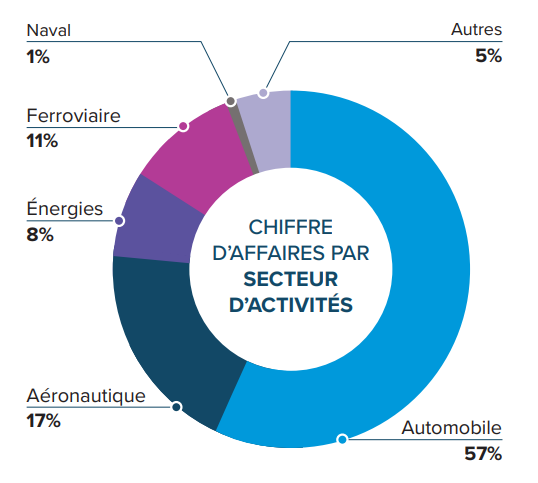
\includegraphics[width=0.5\linewidth]{CA_secteur.png}
    \caption{Répartition du chiffre d’affaires de SEGULA Technologies par secteurs}
\end{figure}

L'activité de SEGULA Technologies s'articule autour de deux axes principaux :
\begin{itemize}
    \item Conseil en technologie et en recherche \& développement
    \item Conseil en organisation et en systèmes d'information
\end{itemize}
\begin{figure}[H]                     
    \centering
    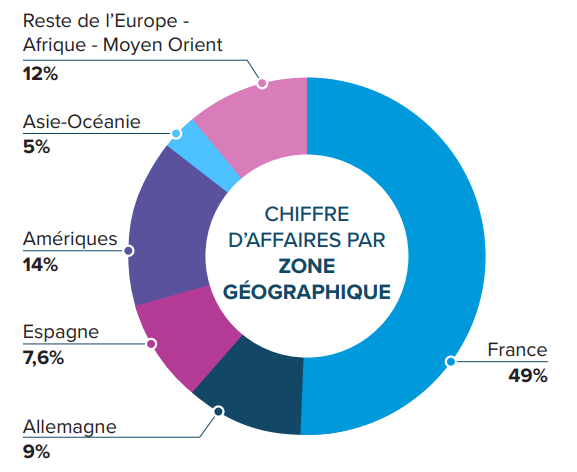
\includegraphics[width=0.5\linewidth]{CA_zone.png}
    \caption{Répartition géographique du chiffre d’affaires de SEGULA Technologies}
\end{figure}

\newpage
\subsection{Secteurs d'activité}
SEGULA Technologies est un groupe d’ingénierie présent à l’échelle internationale, qui ac
compagne la compétitivité des principaux secteurs industriels. Ses interventions couvrent
notamment les domaines de l’automobile, de l’aéronautique, de l’énergie, du rail et du
naval.Lafigure ci-dessous illustre la diversité
des secteurs dans lesquels le groupe opère.
\begin{figure}[H]
    \centering
    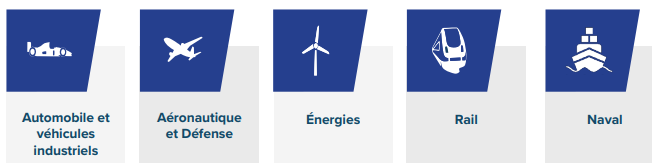
\includegraphics[width=0.5\linewidth]{secteurs.png}
    \caption{Les secteurs d’activitées de SEGULA Groupe}
    \label{fig:placeholder}
\end{figure}
\begin{itemize}
    \item \textbf{Automobile \& Véhicules Industriels} : Présent dans de nombreuses grandes villes à travers le monde, SEGULA Technologies rassemble des milliers de collaborateurs passionnés par le secteur automobile et les véhicules industriels. Les prestations couvrent un large spectre, allant de la gestion de plateformes techniques externalisées à la conception et à l'industrialisation de sous-ensembles.
    \item \textbf{Aéronautique, Aérospatial et Défense} : SIMRA, filiale spécialisée de SEGULA Technologies, a continuellement fait évoluer son offre pour répondre aux exigences croissantes des principaux acteurs des secteurs aéronautique, spatial et de la défense.
    \item \textbf{Énergie} : SEGULA Technologies collabore avec les principaux donneurs d'ordre industriels dans les secteurs de l'énergie nucléaire, thermique et renouvelable.
    \item \textbf{Ferroviaire} : Le groupe apporte son expertise aux industriels du ferroviaire à l'échelle mondiale, intervenant sur l'ensemble du cycle de développement des projets.
    \item \textbf{Naval} : SEGULA Technologies travaille avec les principaux acteurs du secteur naval, couvrant tous types de navires civils, militaires, maritimes et fluviaux.
    \item \textbf{Pétrochimie} : Le groupe soutient les grands donneurs d'ordre du raffinage, de la pétrochimie et de la chimie dès la phase de conception des installations.
    \item \textbf{Pharmacie} : Depuis plus de dix ans, SEGULA Technologies met son expertise au service des principaux acteurs du secteur des sciences de la vie dans leurs projets industriels.
\end{itemize}

\subsection{Clients de SEGULA}
SEGULA Technologies est un acteur majeur de l'ingénierie au service de grands clients industriels. Dans le secteur automobile, Stellantis est reconnu comme l'un de ses principaux partenaires. Le groupe compte également de nombreux autres clients dans les domaines de l'aéronautique, de l'énergie, du ferroviaire et de la pharmacie.

\subsection{SEGULA Technologies Maroc}
\subsubsection{Présentation}
SEGULA Technologies Maroc intervient principalement dans le secteur automobile via ses bureaux d'études situés à Casablanca, Agadir et Tanger, ainsi que dans le secteur aéronautique par l'intermédiaire de sa filiale SIMRA. Dans le domaine automobile, l'entreprise a réalisé de nombreux projets en mode forfaitaire, accompagnant ses clients dans la conception et l'industrialisation de nouveaux produits et la création de nouvelles usines. Dans le secteur aéronautique, SIMRA collabore avec les principaux industriels marocains et internationaux.

\subsubsection{Fiche signalétique de SEGULA Technologies Maroc}
\begin{table}[h!]
    \centering
    \begin{tabular}{|p{4cm}|p{10cm}|}
        \hline
        \textbf{Raison sociale} & SEGULA Technologies Maroc \\ \hline
        \textbf{Forme juridique} & Société Anonyme \\ \hline
        \textbf{Activité} & Groupe d'ingénierie \\ \hline
        \textbf{Date de création} & 2018 \\ \hline
        \textbf{Domaines d'expertise} & Plan de forme Roulage (Kénitra), optimisation des coûts RHN, Conception \\ \hline
        \textbf{Implantations} & - Casablanca Nearshore Park, 1100 Bd. Al Qods, Shore 26, Sidi Maarouf, 20270 Casablanca \newline - Park View Square, La Baie des Palmiers, immeuble 56 Founty, 80010 Agadir \newline - Bureau C1-B, 3e étage, Centre d'Affaires ZF Business Center, lot 40-A, Zone Franche d'Exportation, Tanger \newline - Zone Technopole Aéroport Mohamed V (site de la filiale SIMRA) \\ \hline
        \textbf{Site web} & \url{https://morocco.segulatechnologies.com} \\ \hline
    \end{tabular}
    \caption{Fiche signalétique de SEGULA Technologies Maroc}
\end{table}

\subsubsection{Organigramme de la société}
Une entreprise est une organisation hiérarchique regroupant différentes activités. L'organigramme de SEGULA Technologies Maroc, où s'est déroulé mon stage, est structuré pour permettre une gestion efficace de ses projets.

\subsubsection{Organisation du département « Vehicle Engineering »}
Le département Vehicle Engineering de SEGULA Technologies Maroc joue un rôle central dans le développement de solutions d'ingénierie et de design pour l'industrie automobile. Il regroupe plusieurs équipes spécialisées :

\begin{itemize}
    \item \textbf{Équipe Remontage numérique} : Ce pôle est chargé de la gestion et de la mise à jour des maquettes numériques 3D, base essentielle à la conception et au développement du véhicule. Les ingénieurs assurent la consolidation des données issues des différents sous-systèmes.
    \item \textbf{Équipe Architecture} : Cette équipe est responsable de l'intégration globale des systèmes et sous-systèmes dans le véhicule. Elle prend en compte les contraintes réglementaires, les exigences stylistiques, les contraintes industrielles ainsi que la qualité perçue.
    \item \textbf{Équipe Implantation} : Le pôle Implantation se concentre sur la synthèse géométrique des pièces et sous-systèmes, garantissant leur positionnement optimal dans l'espace véhicule pour éviter les interférences et respecter les règles métier.
\end{itemize}

\section{Contexte général du projet}

\subsection{Problématique}
Dans le secteur du recrutement et des entreprises de services du numérique, la présentation des profils des candidats ou des consultants aux clients finaux revêt une importance capitale. Ce processus implique généralement la conversion des Curriculum Vitae (CV) originaux, souvent hétérogènes en termes de format (documents texte, PDF, images scannées) et de structure, vers un format standardisé propre à l'entreprise, communément appelé "Dossier de Compétences" ou "BioProfile".

Actuellement, cette tâche de transcription et de mise en forme est principalement réalisée de manière manuelle par les équipes des Ressources Humaines (RH) ou les ingénieurs d'affaires. Dans ce cadre dynamique, la gestion et le traitement efficaces de ces documents deviennent cruciaux pour assurer une réactivité commerciale face aux besoins des clients. Mon projet se concentre sur le développement d'un pipeline d'automatisation exploitant l'intelligence artificielle pour traiter ces flux de documents.

Le défi principal réside dans la conception d'un système automatisé qui non seulement ingère et analyse ces données non structurées de manière fiable, mais permet aussi de générer des documents de présentation harmonisés. La problématique se complexifie avec les exigences de précision dans l'extraction des informations clés (compétences, expériences, formations) à partir de formats complexes (tableaux, scans). De plus, l'utilisation de l'intelligence artificielle dans ce domaine nécessite une attention particulière sur la sécurité et la confidentialité des données à caractère personnel, éléments primordiaux dans le secteur du recrutement. La conception du pipeline doit donc être robuste, intelligente et sécurisée pour s'adapter à la diversité des CV reçus.

\subsection{Objectifs de la mission}
Le principal objectif de cette mission est de fournir aux équipes de recrutement et aux ingénieurs d'affaires un outil intelligent leur permettant d'automatiser la création des dossiers de compétences, afin de se concentrer sur des tâches à plus forte valeur ajoutée comme l'évaluation humaine des candidats.

Durant mon projet, j'ai été amenée à :
\begin{enumerate}
    \item Créer un pipeline automatisé d'ingestion et de prétraitement de documents supportant de multiples formats (texte natif et documents scannés).
    \item Implémenter un moteur d'extraction intelligente, basé sur l'intelligence artificielle, capable de comprendre la sémantique d'un CV et d'en extraire les informations pertinentes de manière structurée.
    \item Développer un module de génération automatisée de documents, chargé de formater les données extraites (incluant la photo de profil) dans un modèle de présentation dynamique (PowerPoint).
    \item Concevoir une architecture garantissant le traitement local des données pour assurer une confidentialité et une sécurité totales.
    \item Créer et déployer une interface utilisateur intuitive permettant aux équipes d'interagir facilement avec le système de génération.
\end{enumerate}

\subsection{Enjeux de la mission}
Les enjeux de ce projet sont :
\begin{itemize}
    \item \textbf{Améliorer la productivité :} Favoriser la réactivité commerciale en réduisant drastiquement le temps passé sur des tâches administratives répétitives (la refonte des CV), accélérant ainsi le processus de proposition de profils aux clients.
    \item \textbf{Garantir la sécurité des données :} Assurer la souveraineté et la confidentialité des informations personnelles des candidats en intégrant des modèles d'intelligence artificielle fonctionnant en circuit fermé, répondant ainsi aux normes de sécurité strictes.
    \item \textbf{Standardiser la qualité :} Harmoniser la présentation commerciale des profils de l'entreprise, en éliminant les erreurs humaines liées à la ressaisie et en garantissant un livrable final visuellement irréprochable.
    \item \textbf{Soutenir la transformation digitale :} Contribuer à la modernisation des processus internes des ressources humaines en intégrant des technologies avancées d'analyse de documents et d'intelligence artificielle générative.
\end{itemize}


\section{Planification du projet}

\subsection{Diagramme de GANTT}
Le diagramme de Gantt est l'un des outils les plus efficaces pour faciliter la gestion des projets. Il permet une visualisation claire de l'état d'avancement en spécifiant les dates de début et de fin, ainsi que la durée de chaque tâche. Nous avons utilisé ce diagramme pour la planification complète de notre stage de deux mois (8 semaines). Cette planification resserrée nous a aidé à travailler efficacement et à réaliser le projet dans les délais impartis.

\vspace{1cm}
\begin{figure}[H]
    \centering
    % Ajustement de la taille pour s'adapter à la largeur de la page
    \resizebox{0.95\textwidth}{!}{
    \begin{ganttchart}[
        hgrid,
        vgrid,
        x unit=0.9cm,
        y unit title=0.6cm,
        y unit chart=0.6cm,
        title label font=\bfseries\footnotesize,
        bar label font=\footnotesize,
        group label font=\bfseries\footnotesize,
        bar/.style={fill=blue!50, draw=blue!80, line width=1pt},
        group/.style={fill=gray!80, draw=black},
        progress label text={},
        group right shift=0,
        group top shift=0.6,
        group height=.2,
        group peaks width={0.1}]{1}{8}
        
        \gantttitle{Planification du Projet (8 semaines)}{8} \\
        \gantttitlelist{1,...,8}{1} \\
        
        \ganttgroup{Phase 1 : Analyse \& Besoins}{1}{1} \\
        \ganttbar{Compréhension \& Analyse}{1}{1} \\
        
        \ganttgroup{Phase 2 : Architecture}{2}{2} \\
        \ganttbar{Conception du pipeline}{2}{2} \\
        
        \ganttgroup{Phase 3 : Dév. Extraction \& IA}{3}{5} \\
        \ganttbar{Prétraitement \& OCR}{3}{4} \\
        \ganttbar{Intégration Modèle IA}{4}{5} \\
        
        \ganttgroup{Phase 4 : Génération \& Interface}{6}{7} \\
        \ganttbar{Génération Documentaire}{6}{6} \\
        \ganttbar{Interface Utilisateur}{7}{7} \\
        
        \ganttgroup{Phase 5 : Finalisation}{8}{8} \\
        \ganttbar{Tests, Débogage \& Rapport}{8}{8}
        
    \end{ganttchart}
    }
    \caption{Diagramme de GANTT prévisionnel du projet sur 2 mois}
    \label{fig:gantt_2mois}
\end{figure}
Lors de notre projet, nous avons débuté par une compréhension approfondie de la problématique. Durant la première semaine, nous avons consacré notre temps à analyser les besoins des utilisateurs finaux (équipes RH et commerciaux) et à identifier les défis liés au traitement des CV. Cela impliquait d'examiner les formats de documents reçus et de définir clairement les règles de gestion et les attentes du livrable final.

Ensuite, au cours de la deuxième semaine, nous avons travaillé sur la conception de l'architecture globale du système. Nous avons évalué différentes approches pour l'extraction de texte, la reconnaissance optique de caractères pour les documents scannés, et sélectionné les modèles d'intelligence artificielle les plus adaptés à une exécution locale. Les propositions d'architecture ont été validées pour s'assurer de leur faisabilité sur la durée restante du stage.

Entre la troisième et la cinquième semaine, nous sommes entrés dans la phase principale de réalisation en implémentant le pipeline de prétraitement et d'extraction de données. Cela comprenait le développement des modules permettant de lire les documents, d'isoler les images (comme les photos de profil) et de préparer le texte brut. En parallèle, nous avons configuré et optimisé le moteur d'intelligence artificielle pour qu'il analyse ce texte et restitue les données du candidat sous un format strictement structuré, prêt à être exploité.

Au cours des semaines six et sept, nous nous sommes concentrés sur le module de post-traitement et l'interface utilisateur. Nous avons développé le système chargé de la génération automatisée des présentations, capable d'injecter dynamiquement les données structurées dans le modèle de présentation officiel de l'entreprise. Simultanément, nous avons intégré l'interface web pour rendre ce service accessible et facile d'utilisation pour les équipes métiers.

Enfin, la huitième et dernière semaine a été dédiée à une phase de tests intensifs sur des échantillons réels de CV variés, au débogage final de l'application, et à la rédaction de la documentation et du présent rapport de stage.



\subsection{Méthodologie de réalisation du projet}
La réalisation d'un projet intégrant de l'intelligence artificielle et de l'automatisation de flux documentaires nécessite une méthodologie structurée pour garantir l'atteinte des objectifs métiers. Voici la méthodologie que nous avons adoptée, organisée en plusieurs étapes clés :

\textbf{1. Définition des Objectifs et des Exigences} \\
La première étape consiste à définir clairement les objectifs du projet en termes de résultats et de besoins fonctionnels. Il est essentiel de comprendre quelles informations doivent impérativement figurer sur le document final et comment l'outil s'insérera dans le quotidien des équipes. Cela implique de documenter les exigences de performance, de tolérance aux différents formats de fichiers, et surtout les contraintes strictes de sécurité et de confidentialité des données.

\textbf{2. Analyse et Compréhension des Données} \\
Cette étape implique de recenser et d'analyser la nature des données d'entrée (les CV). Il a fallu examiner la structure, la variabilité des mises en page, l'utilisation de tableaux ou de colonnes, et la présence de documents non textuels (scans). Cette exploration permet d'identifier les limites des méthodes d'extraction classiques et de planifier la mise en place d'outils avancés de vision par ordinateur pour pallier ces problématiques de qualité de données.

\textbf{3. Conception de l'Architecture du Pipeline} \\
À ce stade, il a fallu concevoir un flux de traitement des données adapté aux besoins du projet. Le modèle a été pensé de manière modulaire : un module d'ingestion (lecture multiformat), un module d'intelligence artificielle (analyse sémantique et structuration), et un module de restitution (génération du document final). Chaque choix technologique a été évalué en fonction de sa capacité à fonctionner de manière autonome et sécurisée, sans dépendre de services externes non maîtrisés.

\textbf{4. Développement et Mise en Œuvre} \\
Cette étape correspond à la phase de programmation des processus automatisés. Les développements ont inclus l'écriture des algorithmes de lecture, la mise au point des directives (prompts) envoyées au modèle d'intelligence artificielle pour garantir la précision de l'extraction, ainsi que le développement de la logique d'injection des données dans la présentation cible. Des tests unitaires continus ont été réalisés pour s'assurer que chaque composant du pipeline fonctionnait correctement de manière isolée.

\textbf{5. Déploiement et Interface Utilisateur} \\
Une fois les algorithmes validés, le pipeline a été intégré au sein d'une interface web. Le déploiement s'est fait de manière à rendre l'outil accessible via un simple navigateur, dissimulant la complexité technologique sous-jacente. Il est également essentiel à cette étape de s'assurer de la stabilité du service pour gérer plusieurs requêtes simultanées de la part des utilisateurs.

\textbf{6. Tests, Évaluation et Optimisation} \\
Mettre en place des tests d'intégration complets sur des cas réels (Edge cases) est crucial. En fonction des retours qualitatifs obtenus lors des premiers essais, les algorithmes de détection et les instructions du modèle d'IA ont été ajustés. L'optimisation continue permet d'assurer que le système reste robuste face à l'infinie variété de présentations possibles d'un CV.


\section{Conclusion}
Ce chapitre a posé le cadre général de notre projet de fin d'année, en mettant en lumière les défis liés à la gestion documentaire dans le secteur du recrutement et de l'ingénierie. La refonte manuelle des CV en dossiers de compétences est une tâche chronophage qui freine la réactivité des équipes. Nous avons défini les objectifs de notre mission, visant à créer un écosystème automatisé capable d'analyser intelligemment ces documents et de générer des présentations standardisées, tout en répondant aux enjeux critiques de sécurité des données.

La planification rigoureuse du projet et l'adoption d'une méthodologie modulaire ont permis de structurer notre approche, allant de la compréhension initiale des données non structurées jusqu'au déploiement d'une interface utilisateur intuitive.

À la lumière de cette étude du contexte et des objectifs fixés, il devient évident que pour relever ces défis d'extraction et de génération automatisée, l'intégration de technologies avancées de traitement du langage naturel et d'analyse d'images est cruciale. Le prochain chapitre se penchera sur l'état de l'art des concepts et des technologies de pointe pouvant aider à résoudre ces problématiques, en optimisant la performance de notre pipeline documentaire et en garantissant la qualité des données extraites.
